% Fuentes que no vi:
% https://www.youtube.com/@AuxiRolando
\documentclass[a4paper]{article}
\usepackage[margin=1.5cm]{geometry}
%\documentclass[11pt]{article}
%\usepackage[paperwidth=9cm,paperheight=60cm,margin=0.4cm]{geometry}
\usepackage{multicol}
\usepackage{enumitem}
\usepackage{graphicx}
%Links
\usepackage[colorlinks = true,
            linkcolor = blue,
            urlcolor  = blue,
            citecolor = blue,
            anchorcolor = blue]{hyperref}
%Simbolos matemáticos
\usepackage{amsmath}
\usepackage{amssymb}
%Manejo de argumentos en los comandos
\usepackage{xparse}
%Enumeracion
\usepackage{enumitem}
%Páginas sin numeración
\pagestyle{empty}
%Interlineado
\renewcommand{\baselinestretch}{1.5}
%Arreglar comillas
\usepackage [autostyle]{csquotes}
\MakeOuterQuote{"}
%Macros
\newcommand{\Item}{\item[\stepcounter{enumii}$\blacktriangleright$\textbf{(\alph{enumii})}]} %Negrita en algunos items
\newcommand{\answer}{\item[**]}
\newcommand{\exercise}{\item}
%Logic macros
\newcommand{\then}{\to}
\newcommand{\eq}{\leftrightarrow}
\newcommand{\xor}{\veebar}
\newcommand{\nor}{\downarrow}
\newcommand{\nimply}{\nrightarrow}
\newcommand{\nand}{\uparrow}
\newcommand{\Then}{\Rightarrow}
\newcommand{\Eq}{\Leftrightarrow}
\newcommand{\intersec}{\cap}
\newcommand{\union}{\cup}
\newcommand{\Delta}{\symdiff}
\newcommand{\compl}[1]{\overline{#1}}
\newcommand{\df}[2]{\displaystyle\frac{#1}{#2}}
% Command to format each premise or reasoned proposition
\NewDocumentCommand{\FormatItem}{m}{%
    #1 \\[-4pt]
}
% Define the \Reasoning command
\NewDocumentCommand{\Reasoning}{>{\SplitList{;}}m m}{%
    \begin{minipage}[t]{\linewidth}
    \ProcessList{#1}{\FormatItem} % Process each premise
    \\[-24pt] \hspace{-.5cm}\rule[.5pt]{2.2cm}{.5pt}\\[-8pt]
    #2 \\[-8pt]% This is the conclusion
    \end{minipage}%
}
% Define the \DReasoning command
\NewDocumentCommand{\DReasoning}{>{\SplitList{;}}m >{\SplitList{;}}m m}{%
    \begin{minipage}[t]{\linewidth}
    \ProcessList{#1}{\FormatItem} % Process each premise
    \\[-24pt] \hspace{-.5cm}\rule[.5pt]{3cm}{.5pt}\\[-8pt]
    \ProcessList{#2}{\FormatItem} % Process each reasoned proposition
    \\[-24pt] \hspace{-.5cm}\rule[.5pt]{3cm}{.5pt}\\[-8pt]
    #3 \\[-8pt]% This is the conclusion
    \end{minipage}%
}
\begin{document}
\noindent \hrulefill 
\vspace{-7pt}
\begin{center} 
	\textbf{ Práctica 2: Teoría de conjuntos} \\
	Comisión: Rodrigo Cossio-Pérez y Leonardo Lattenero
\end{center}
\vspace{-10pt}
\hrulefill \\
\phantom{~} \\
%\textbf{EJERCICIOS JR.}
\begin{enumerate}
	\exercise Dados los conjuntos \\ $A=\{a,b\}$ ~~~~~~~~ $B=\{ \{a\}, \{b\} \}$ ~~~~~~~~ $C=\{ \{a\}, b, \{b\}, \{a,b\} \}$ \\ analizar cuáles de las siguientes afirmaciones son verdaderas:
	\begin{multicols}{3}
	\begin{enumerate} [label=(\alph*)]
		\item $A=B$
		\item $A \subseteq C$
		\item $\{b\} \in C$
		\item $\{a,b\} \in A$
		\item $a \in C$
		\item $\{b\} \in B$
		\item $\{b\} \subseteq B$
		\item $\{a\} \in A$
		\item $\{a\} \subseteq A$
		\item $\{b\} \subseteq C$
	\end{enumerate}
	\end{multicols}
	\exercise Dados los conjuntos \\ $A=\{1,2,3\}$ ~~~~~~~~ $B=\{ \{2,3\}, 1, 4\}$ ~~~~~~~~ $C=\{ 2,3,4 \}$ ~~~~~~~~ $D=\{ \{1,2,3\} ,4 \}$ \\ hallar los conjuntos: 
	\begin{multicols}{3}
	\begin{enumerate} [label=(\alph*)]
		\item $A\setminus B$
		\item $(A \setminus B) \union C$
		\item $(A \union B) \setminus (C \intersec D)$
		\item $A \symdiff C$
		\item $\compl{A}$ considerando el universo $U=\mathbb{N}$
	\end{enumerate}
	\end{multicols}
	\exercise Determinar la unión e intersección de los siguientes pares de intervalos reales: 
	\begin{multicols}{3}
	\begin{enumerate} [label=(\alph*)]
		\item $A=\left[-2;7\right]$  y $B=\left(0;10\right]$
		\item $A=\left[-2;\df{5}{3}\right]$  y $B=\left(-1;1\right]$
		\item $A=\left(-\infty;\df{1}{2}\right)$  y $B=\left[-12;\pi \right]$
		\item $A=\left[-5;4\right]$  y $B=\left[9;12\right]$
	\end{enumerate}
	\end{multicols}
	%\begin{center}
	%	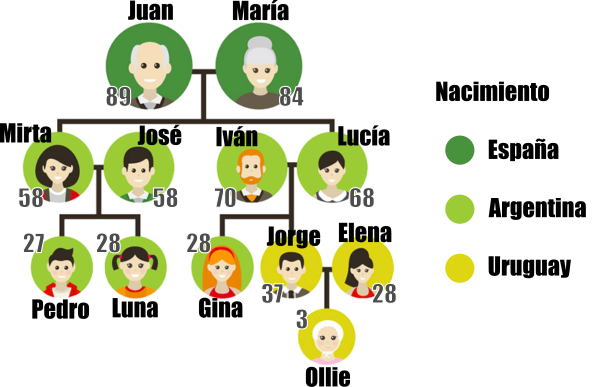
\includegraphics[height=5cm]{familia.png}
	%\end{center}
\end{enumerate}
\vspace{20pt} 
 \textbf{RESPUESTAS}\begin{enumerate}\exercise\begin{enumerate} [label=(\alph*)]		\item Falso
		\item Falso
		\item Verdadero
		\item Verdadero
		\item Falso
		\item Verdadero
		\item Falso
		\item Falso
		\item Verdadero
		\item Verdadero
\end{enumerate}\exercise\begin{enumerate} [label=(\alph*)]		\item $\{2,3\}$
		\item $\{2,3,4\}$
		\item \{1,2,3,\{2,3\}\}
		\item $\{1,4\}$
		\item $\{ x \in \mathbb{N} ~|~ x \geq 4 \}\{4,5,6,7,8,9,10,11, \cdots \}$
\end{enumerate}\exercise\begin{enumerate} [label=(\alph*)]		\item $A \union B = [-2;10]$ y $A \intersec B = (0;7]$
		\item $A \union B = \left[-2;\df{5}{3}\right]$ y $A \intersec B = \left(-1;\df{5}{3}\right]$
		\item $A \union B = (-\infty;\pi]$ y $A \intersec B = \left(-12;\df{1}{2}\right)$
		\item $A \union B = [-5;4] \union [9;12]$ y $A \intersec B = \emptyset$
\end{enumerate}\end{enumerate}\end{document}